
We have analyzed the microbiome temporal variability to extract global properties of the system. As fluctuations in total counts are plagued by systematic errors we worked on temporal variability of relative abundances for each taxon. Our first finding was that, in all cases, changes in relative abundances of taxa follow a ubiquitous pattern known as the fluctuation scaling law\cite{fs} or Taylor's power law\cite{taylor}, i.e., microbiota of all detected taxa follows $\sigma_i  = V\cdot x_i^{\beta}$, a power law dependence between mean relative abundance $x_i$ and dispersion $\sigma_i$. The law seem to be ubiquitous, spanning even to six orders of magnitude in the observed relative abundances. As can be seen in Figure \ref{fig:main1}, the most abundant species are less volatile in relative terms than the less abundant. The fitting to the power law is always robust ($R^{2}$ > 0.88) and does not depend on the microbiome condition. The power law (or scaling) index $\beta$ and the variability $V$ (hereafter Taylor parameters) appear to be correlated with the stability of the community and related with the health status of the host, which we consider the main finding exposed in this article.

\begin{figure}
	\centering
	\vspace*{-15mm} % Corrects overbox of the figures
	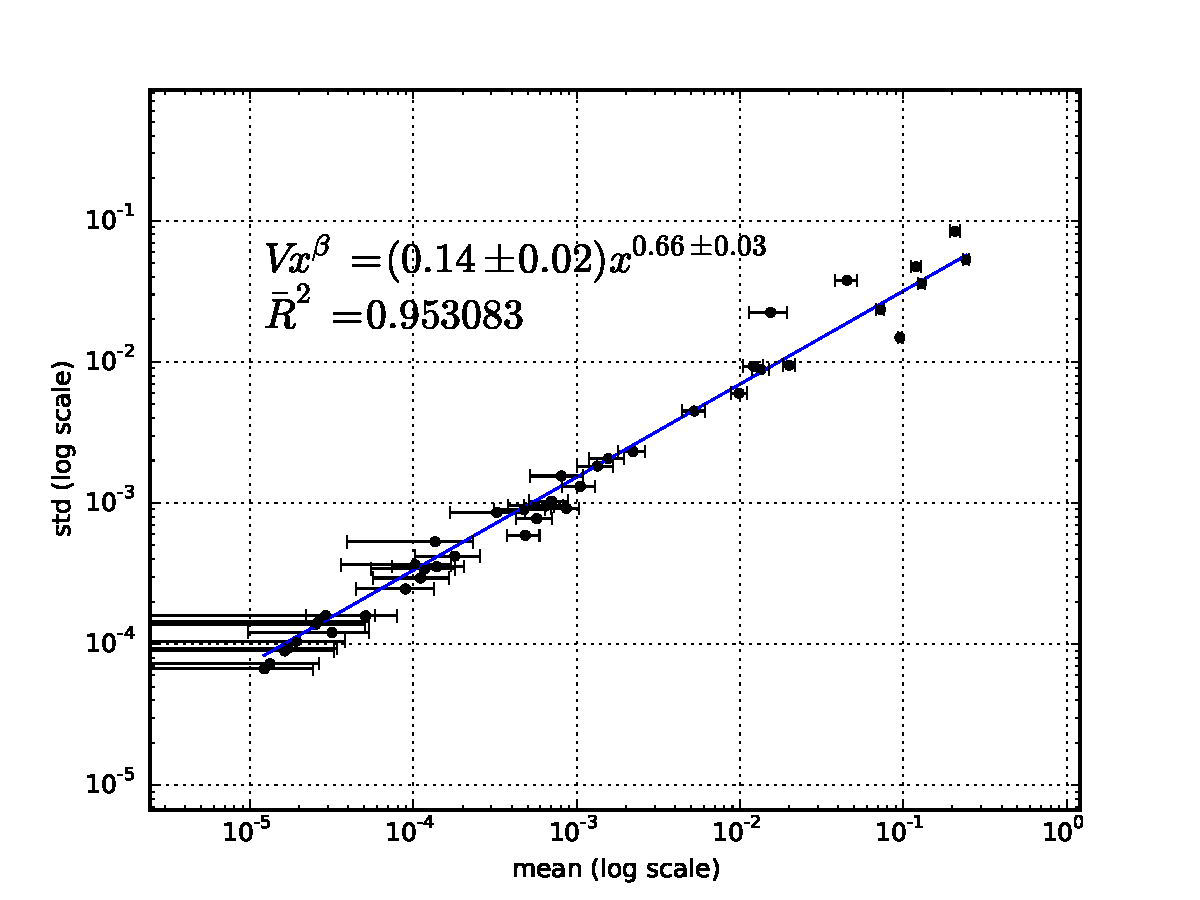
\includegraphics[width=0.8\textwidth]{results/fits/IBS_h_A_amplicons_family_stdVSmean_xWboot_LOG.pdf}
	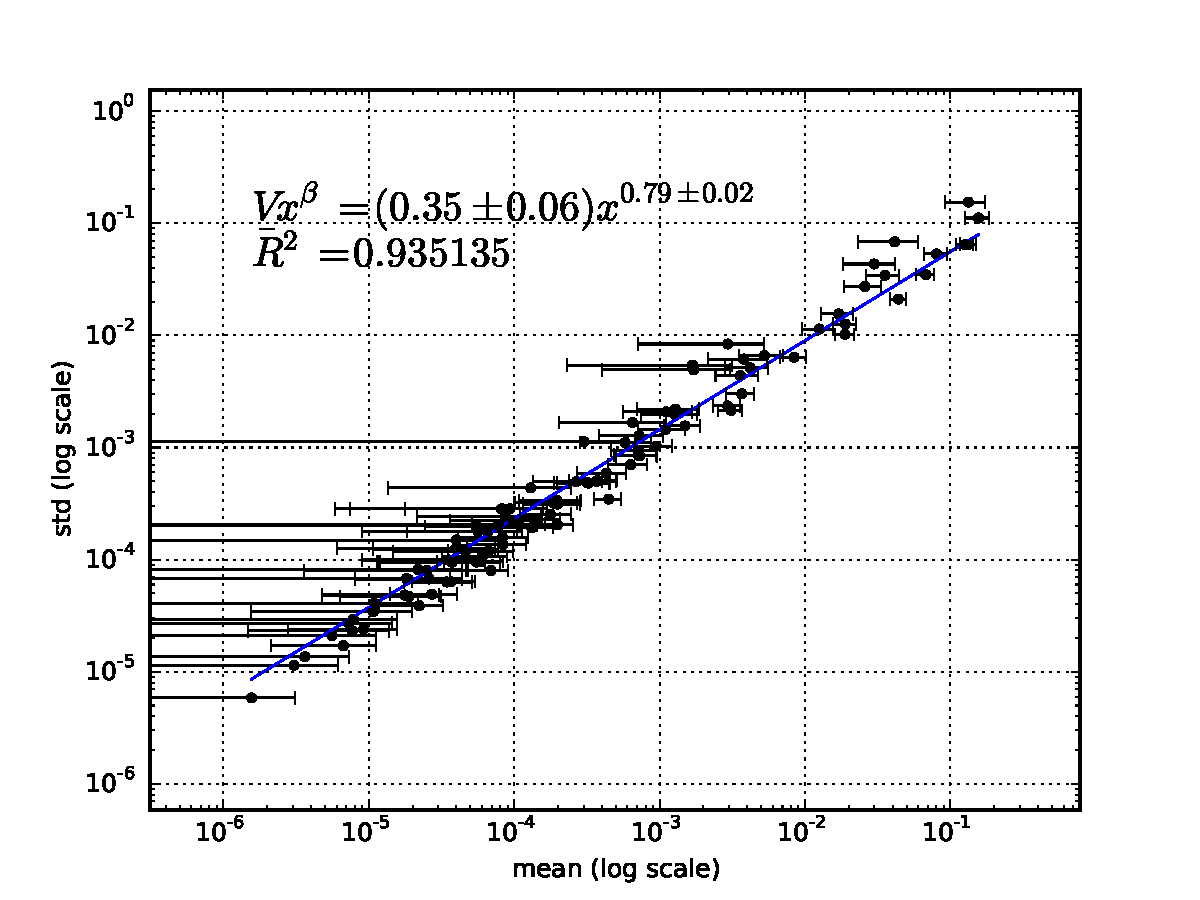
\includegraphics[width=0.8\textwidth]{results/fits/IBS_P2_Metatranscriptores_stdVSmean_xWboot_LOG.pdf}
	\caption{X-weighted power-law fits of the standard deviations versus the mean values for each bacterial genus monitored in time. We show the fit for samples from a healthy subject (top) and from a subject diagnosed with irritable bowel syndrome (bottom), studied in our lab \cite{IBS}. Taylor's power law seems to be ubiquitous, spanning to six orders of magnitude.}
	\label{fig:main1}
\end{figure}

Taylor parameters describing the temporal variability of the gut microbiome in our sampled individuals are shown in Tables S1 to S6. Our results hint at an ubiquitous behavior. On the first hand, the variability (which corresponds to the maximum amplitude of fluctuations) is large, which suggests resilient capacity of the microbiota. On the other hand, the scaling index is always smaller than one, which means that more abundant taxa are less volatile than less abundant ones. In addition, Taylor parameters for the microbiome of healthy individuals in different studies are compatible within estimated errors. This enables us to define an area in the Taylor parameter space that we called the \emph{healthy zone}. % should be changed for any other name: stable zone? 

In order to jointly visualize and compare the results of individuals from different studies, their Taylor parameters have been standardized, where standardization means that each parameter is subtracted by the mean value and divided by the standard deviation of the group of healthy individuals for each study (for details of the procedure, please see Standardization subsection in Material and Methods). The healthy zone and the standardized Taylor parameters for individuals whose gut microbiota is altered (i.e., suffering from kwashiorkor, altered diet, antibiotics or IBS) is shown in Figure \ref{fig:main2}. Children developing kwashiorkor show smaller variability than their healthy twins. A meat/fish-based diet increases the variability significantly when compared to a plant-based diet. All other cases presented increased variability, which is particularly severe, and statistically significant at more than 95\% CL, for obese patients grade III on a diet, individuals taking antibiotics or IBS--diagnosed patients. A global property emerges from all worldwide data collected: Taylor parameters characterize the statistical behavior of microbiome changes. Furthermore, we have verified that our conclusions are robust to systematic errors due to taxonomic assignment (see Figure Sx in Supplemental Material).

\begin{figure}
	\centering
	\includegraphics[width=0.9\textwidth]{results/finalplot11.pdf}
	\caption{Taylor's law parameter space. We have compiled here all the data studied in this work. The coloured circle corresponds to 68\% confidence level (CL) region of healthy individuals in the Taylor parameter space, while dashed line delimites the 98\% CL region. Points with errors place each individual gut microbiome in the Taylor space. Note that the parameters have been standardized (stdev units) to the healthy group in each study for demonstrative and comparative purposes.}
	\label{fig:main2}
\end{figure}

Taylor's power law has been explained in terms of various effects, all without general consensus. It can be shown to have its origin in a mathematical convergence similar to the central limit theorem, so virtually any statistical model designed to produce a Taylor law converge to a Tweedie distribution\cite{stat}, providing a mechanistic explanation based on the statistical theory of errors\cite{convergence1,convergence2,convergence3}. To unveil the generic mechanisms that drive different scenarios in the $\beta$--$V$ space, we model the system by assuming that taxon relative abundance follows a Langevin equation with, on the one hand, a deterministic term that captures the fitness of each taxon and, on the other hand, a randomness term associated with Gaussian random noise\cite{ranking}. Both terms are modeled by power laws, with coefficients that can be interpreted as the taxon fitness $F_i$ and the variability $V$ (see Model under Material and Methods). In this model, when $V$ is sufficiently low, abundances are stable in time. Differences in variability $V$ can induce a noise-induced phase transition in relative abundances of taxa. The temporal evolution of the probability of a taxon having abundance $x_i$ given its fitness is governed by the Fokker--Planck equation. The results of solving this equation show that the stability is best captured by a phase space determined by fitness $F$ and amplitude of fluctuations $V$ (see Figure \ref{fig:main3}). 

\begin{figure}
	\centering
	\vspace*{-5mm} % Corrects overbox of the figures
	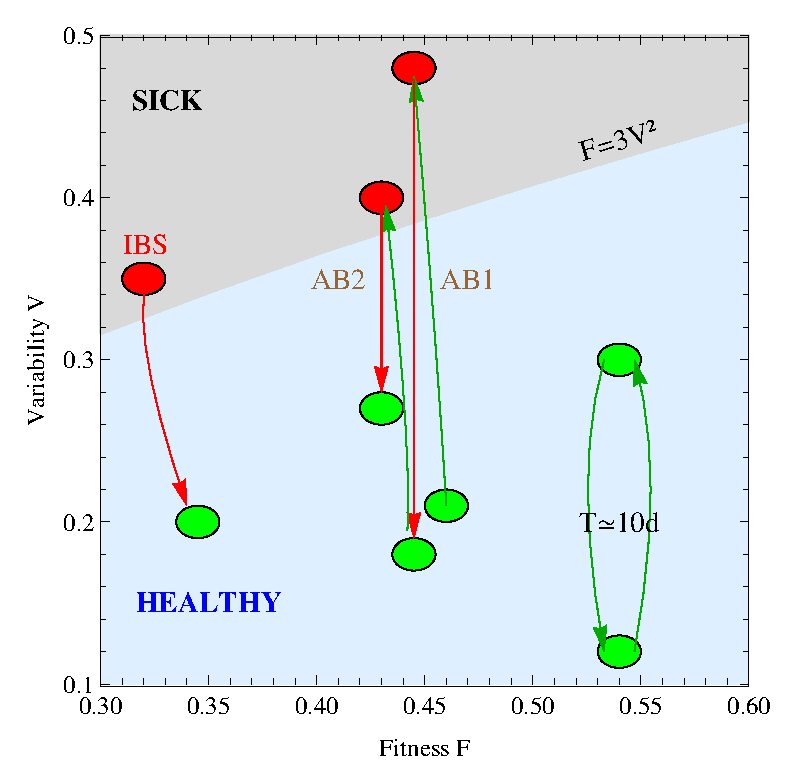
\includegraphics[width=0.8\textwidth]{results/finalPlot33_new.pdf}
	\caption{Microbiota states can be placed in the phase space $F$--$V$. The light blue shaded region corresponds to the stable phase, while the grey shaded region is the unstable phase (the phase transition line is calculated for  $\alpha$ = $\beta$ = 0.75). We place healthy individuals (green) and individuals whose gut microbiota is threatened (antibiotics, IBS) in the phase space fitness--variability. Gut microbiota of healthy individuals over a long term span show a quasi--periodical variability (central period is ten days). We show that taking antibiotics (AB1 and AB2 correspond to first and second treatment respectively) induces a phase transition in the gut microbiota, which impacts its future changes. We also show an IBS--diagnosed patient transiting from the unstable to the stable phase.}
	\label{fig:main3}
\end{figure}

The model predicts two phases for the gut microbiome: a stable phase with large variability that permits some changes in the relative abundances of taxa; and an unstable phase with larger variability, above the phase transition, where the order of abundant taxa varies significantly with time. The microbiome of all healthy individuals was found to be in the stable phase, while the microbiome of several other individuals was shown to be in the unstable phase. In particular, individuals taking antibiotics and IBS--diagnosed patient P2 had the most severe symptoms. In this phase diagram, each microbiota state is represented by a point at its measured variability $V$ and inferred fitness $F$. The model predicts high average fitness for all taxa, i.e., taxa are narrowly distributed in F. The fitness parameter has been chosen with different values for demonstrative purposes. Fitness is larger for the healthiest subjects and smaller for the IBS--diagnosed patients.

%%%
\subsection*{Rank stability of the taxa} 
The rank dynamics and stability plot in Figure \ref{fig:corrank} shows the variation in the rank with time for the most dominant taxa and their calculated Rank Stability Index (RSI, as discussed in Material and Methods) for the taxa of a healthy subject (individual \emph{A}, top) and from a subject diagnosed with IBS (patient \emph{P2}, bottom) of the IBS study\cite{IBS}. The taxa are listed ordered by the accumulated frequency along the time series, so y-axis is an overall dominance axis for each sample set. Generally speaking, we observe that the most dominant taxa are the most rank stable. 

\begin{figure}
	\centering
	\vspace*{-10mm} % Corrects overbox of the figures
	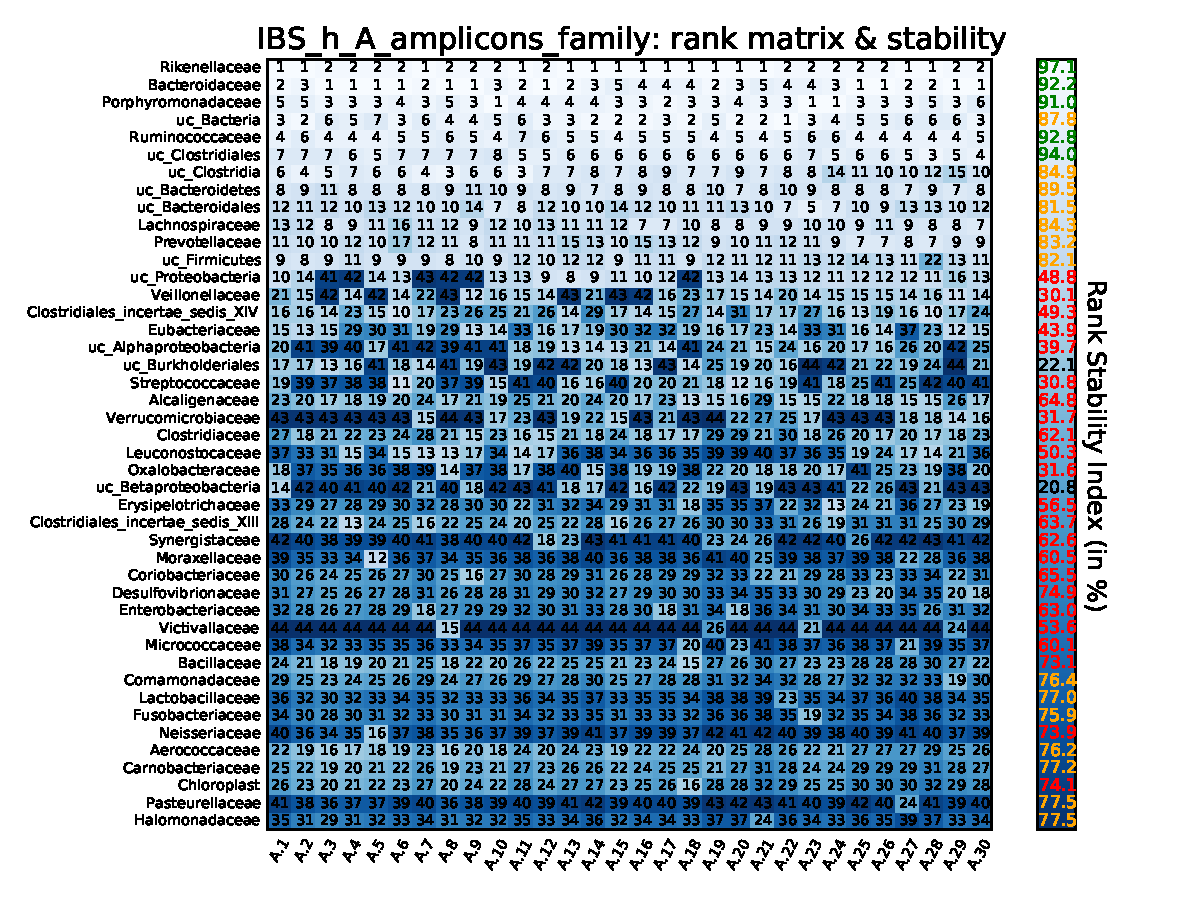
\includegraphics[width=0.8\textwidth]{results/corrank/IBS_h_A_amplicons_family_Rank.pdf}\vspace*{-3mm} % Corrects overbox of the figures
	\hspace*{-4.5mm}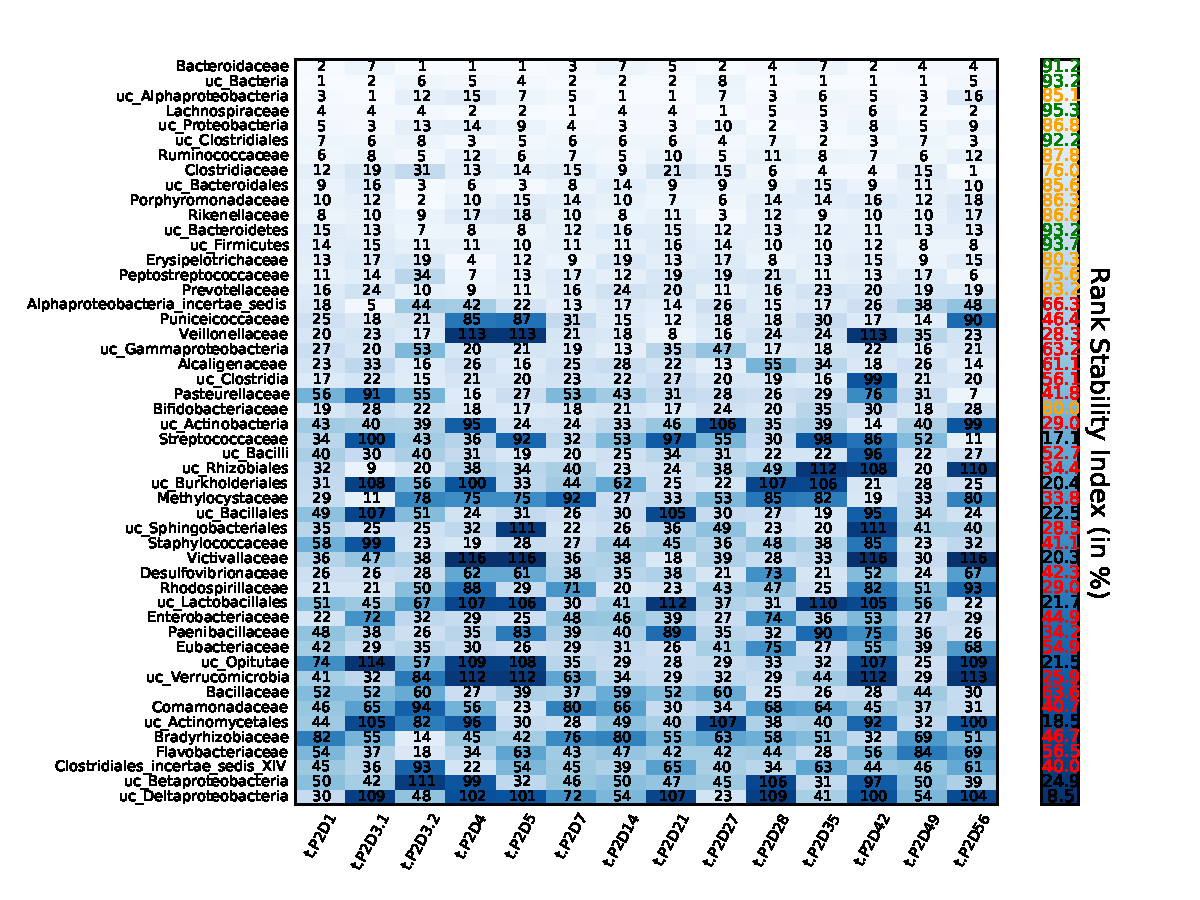
\includegraphics[width=0.83\textwidth]{results/corrank/IBS_P2_Metatranscriptores_Rank.pdf}
	\caption{Matrixes showing the rank variation throughout time for the most dominant elements (taxa) and their calculated Rank Stability Index (as shown in Material and Methods). We show the matrix for samples from a healthy subject (top) and from a subject diagnosed with irritable bowel syndrome (bottom), studied in our lab\cite{IBS}.}
	\label{fig:corrank}
\end{figure}

Nevertheless, in the particular case of the healthy individual, \emph{Burkholderiales} and \emph{Betaproteobacteria} (taxa ordered as 18th and 25th in the dominance axis) show comparatively very low rank stability regarding similar dominant taxa while, on the other hand, \emph{Comamonadaceae}, \emph{Lactobacillaceae}, \emph{Fusobacteriaceae}, \emph{Aerococcaceae} and \emph{Carnobacteriaceae} show higher stability than other more dominant taxa, forming a kind of \emph{rank stability island} for medium-ranked taxa around position 40 in the dominance axis, and thus colored in orange following Table \ref{tab:RSI} criteria, since they show a moderately stable RSI.

\begin{table}
  \begin{center}
    \begin{tabular}{cccr}
    \hline
    Case  &  Condition  &  Colour  &  Description \\
    \hline
    1  &  $1\ge{\rm RSI}>0.99$  & \textcolor{blue}{blue} & constant rank \\ 
    2  & ${\rm RSI}>0.90$  &  \textcolor{green}{green}  & highly stable rank \\
    3  &  ${\rm RSI}>0.75$  &  \textcolor{orange}{orange} & moderately stable rank \\
    4  &  ${\rm RSI}>0.25$  &  \textcolor{red}{red} & unstable rank \\
    5  &  $0.25\ge{\rm RSI}\ge0$  &  \bfseries{black} & very unstable rank \\
    \hline
    \end{tabular}
  \end{center} 
  \caption{Colour code of the RSI percentage text following the first condition satisfied.}
  \label{tab:RSI}
\end{table}

In the IBS diagnosed patient, beyond the differences in dominance for the particular taxa, we still observe that the most dominant are the most rank stable. However, as opposed to the healthy individual results, far from presenting a \emph{rank stability island}, the medium-ranked taxa are very rank unstable, mostly due to transient (often one or two consecutive samples) but deep drops in their relative abundance, which are usually happening more than twice along the time series. That is, for instance, the case of \emph{Sphingobacteriales} with two non-consecutive samples dropping to 111th rank position. In other cases, the high rank instability comes from a rank fluctuation over all the time series, as for \emph{Streptococcaceae} and \emph{Burkholderiales}, which are ranking 26th and 29th respectively in the overall dominance axis but show very low RSI, and thus colored in black attending to Table \ref{tab:RSI}.

We found the presence of such of \emph{rank stability island} for medium-ranked taxa in the other healthy subjects (\emph{B} and \emph{C}) of the IBS study\cite{IBS} together with its total absence for the other IBS diagnosed patient (patient \emph{P1}), which also presents very high rank instability in its medium-ranked taxa.


%%%
\subsection*{Time dependence of model parameters}

Finally, we have studied the time dependence of the variability $V$ and power law index $\beta$ (see Model under Material and Methods) by using a sliding window approach. The total number of time points are divided in subsets of five points, where the next subset is defined by adding the next time sampling and by eliminating the earliest one. Both parameters were calculated for each subset against the average time lapse. Figure \ref{fig:tempevo1} shows the variability  $V$ as a function of time for the largest sampling: two individuals in the Caporaso's study\cite{moving} corresponding to the gut microbiota of a male (upper plot) and a female (lower plot). Figure \ref{fig:tempevo2} shows the time evolution of $V$ for patient P2 of the IBS study\cite{IBS} (upper plot) and patient D in the antibiotics study\cite{antibiotic} (lower plot). Both samples shows changes in the variability V with quasi--periodic behavior peaked at about 10 days. Variability grows more for the gut microbiota of the male and share a minimal value around 0.1 with the gut microbiota of the female. The variability of the gut microbiota of P2 decreases from above 0.3 to below 0.2, showing a slow tendency to increase the order of the system.  Antibiotic intake leaks to a quick increase of variability which lasts for a few days to recover ordering. The second antibiotic treatment shows some memory (lower increase of variability) with a slower recovery.

\begin{figure}
	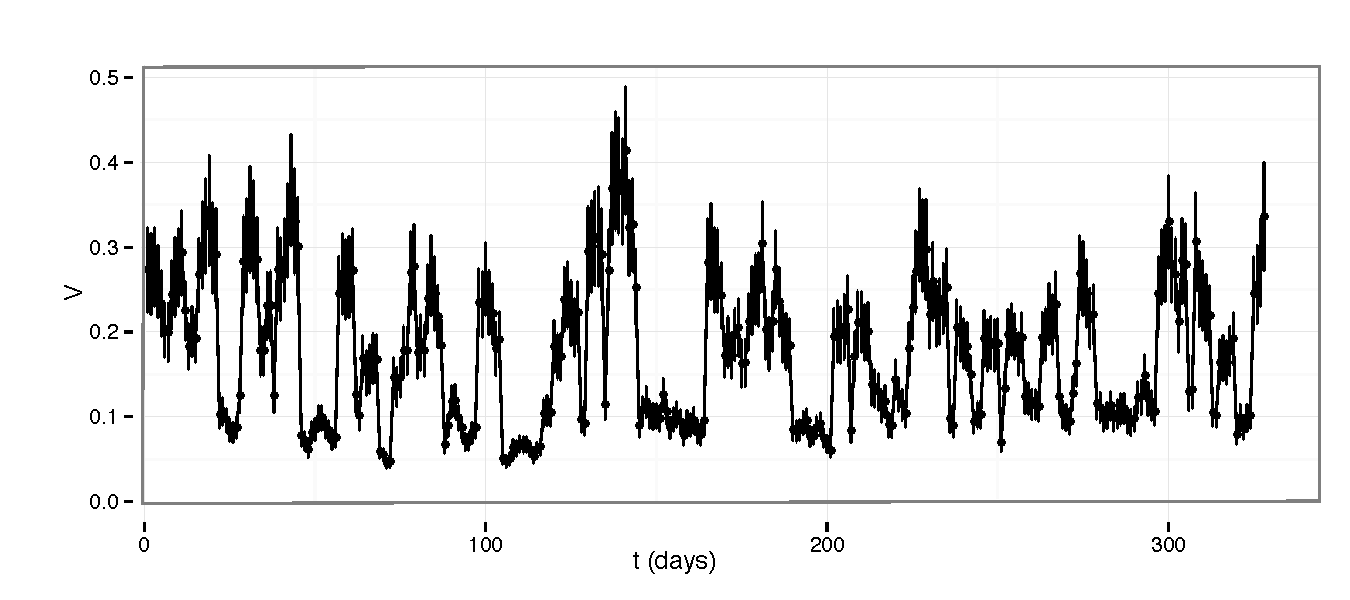
\includegraphics[width=1.0\textwidth]{results/sliwin/male_mov.pdf}
	\hspace*{3mm}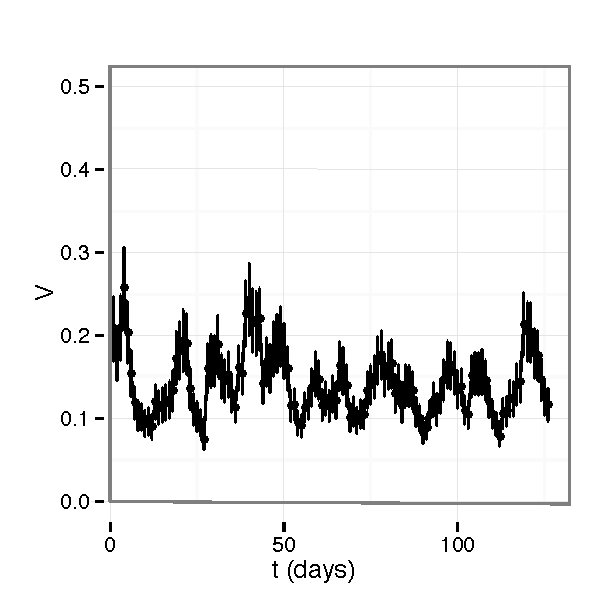
\includegraphics[width=0.448\textwidth]{results/sliwin/female_mov.pdf}
\caption{$V$ as a function of time for the two individuals in the Caporaso's study\cite{moving}: samples of gut microbiome of a male (upper plot) and a female (lower plot).}
\label{fig:tempevo1}
\end{figure}

\begin{figure}
	\centering 
 	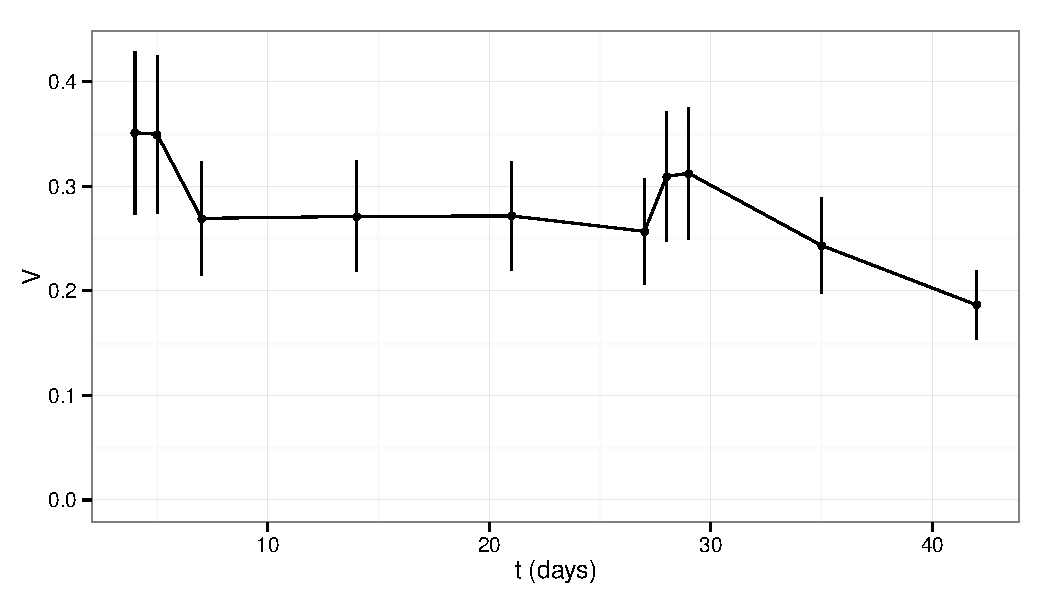
\includegraphics[width=0.8\textwidth]{results/sliwin/patP2_IBS.pdf}
  	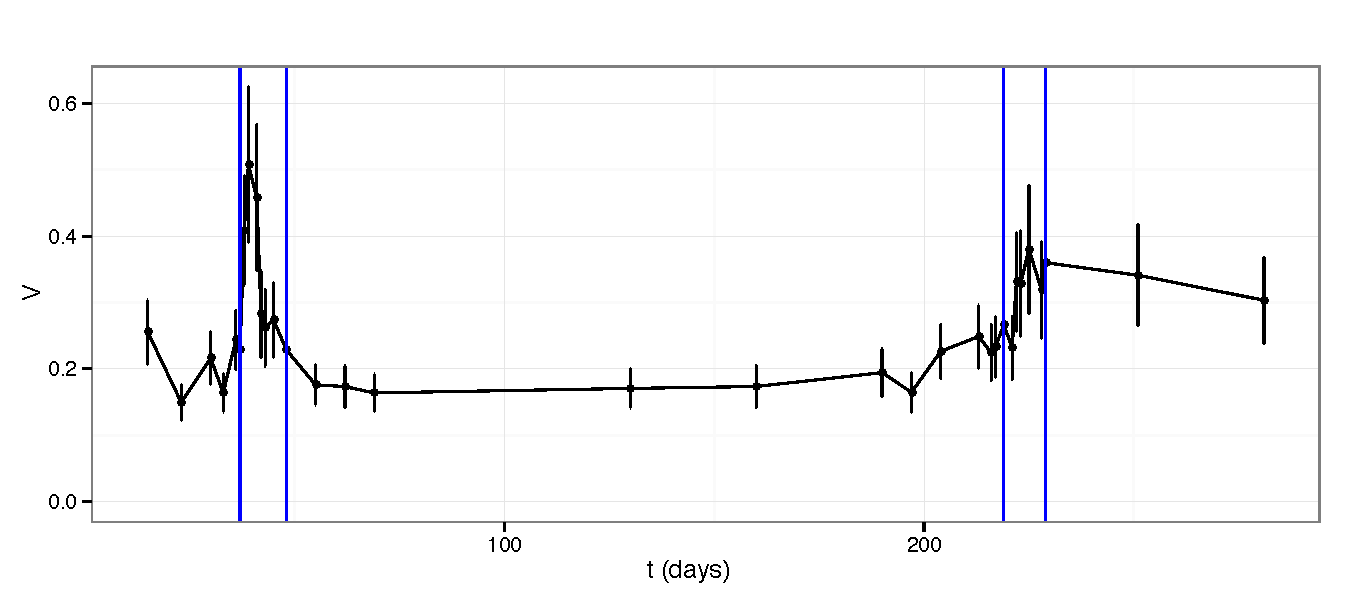
\includegraphics[width=1.0\textwidth]{results/sliwin/patD_antibio.pdf} 
\caption{$V$ as a function of time for patient P2 of the IBS study\cite{IBS} (upper plot) and patient D in the antibiotics study\cite{antibiotic} (lower plot). The blue vertical lines in the lower plot are showing the periods of antibiotic treatment.}
\label{fig:tempevo2}
\end{figure}
